\chapter{Experiments}\label{chapter:experiment}

\section{Case studies}
\paragraph{Dijkstra’s algorithm for mutual exclusion}
\paragraph{Dijkstra’s algorithm for mutual exclusion with a token}
\paragraph{Other mutual exclusion algorithms}
\paragraph{Dining philosophers}
\paragraph{Cache coherence protocols}
\paragraph{Termination detection}
\paragraph{Dining cryptographers}
\paragraph{Leader election}
\paragraph{Token passing}

\section{Results}

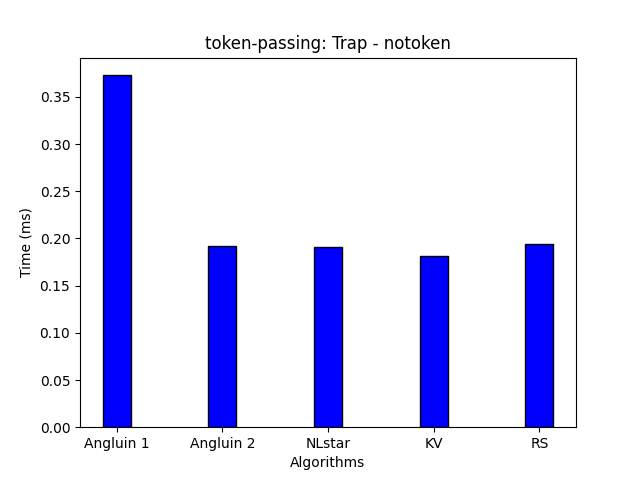
\includegraphics[scale=0.5]{figures/Trap_notoken.png}
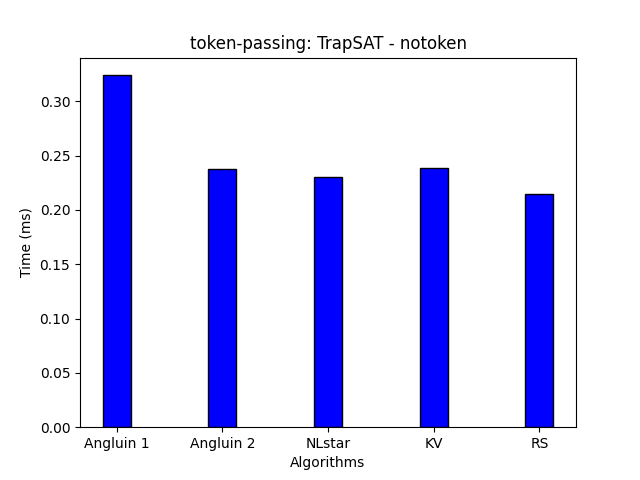
\includegraphics[scale=0.5]{figures/TrapSAT_notoken.png}

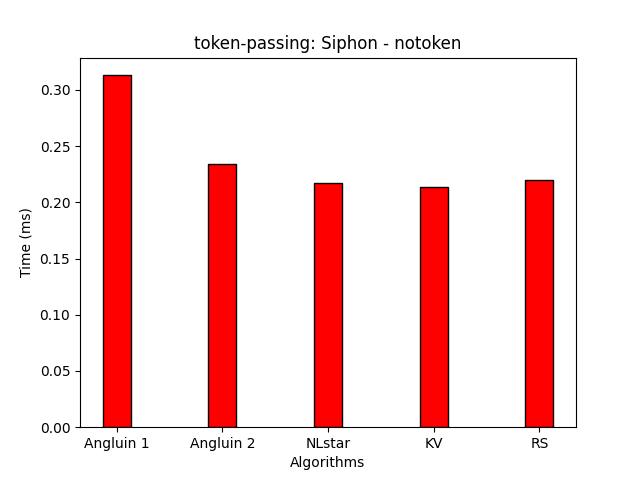
\includegraphics[scale=0.5]{figures/Siphon_notoken.png}
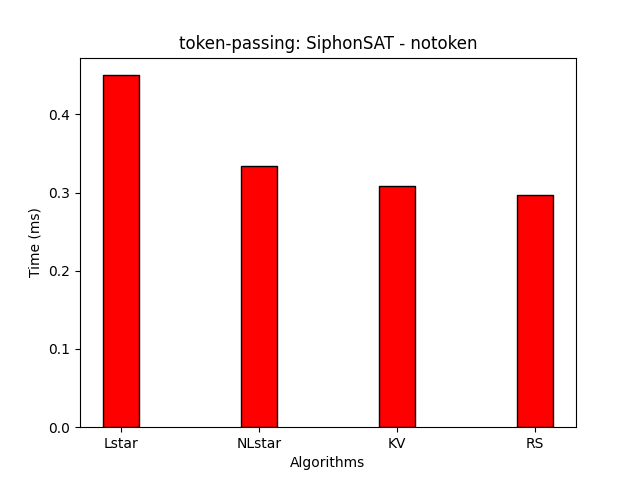
\includegraphics[scale=0.5]{figures/SiphonSAT_notoken.png}

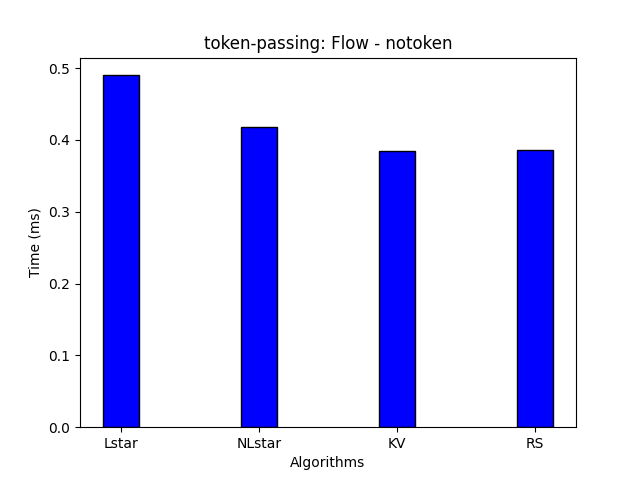
\includegraphics[scale=0.5]{figures/Flow_notoken.png}


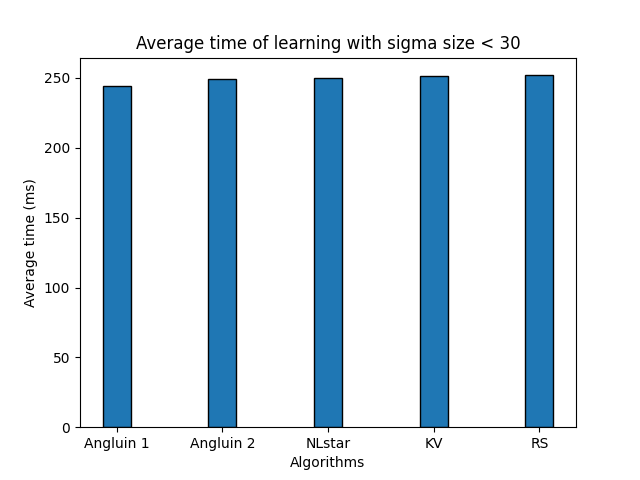
\includegraphics[scale=0.75]{figures/average_time2.png}

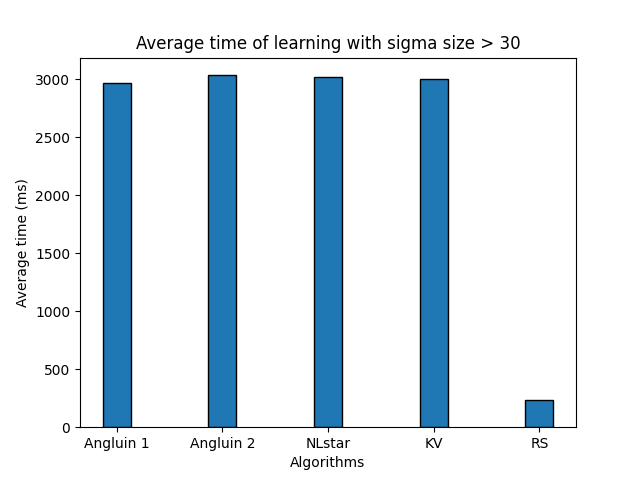
\includegraphics[scale=0.75]{figures/average_time3.png}



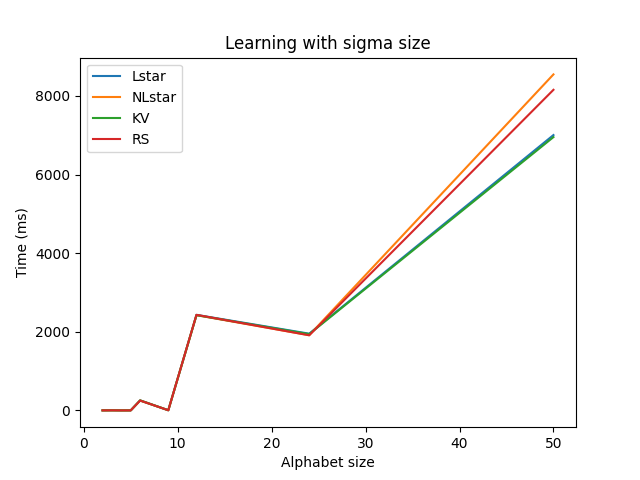
\includegraphics[scale=0.75]{figures/sigma_size.png}

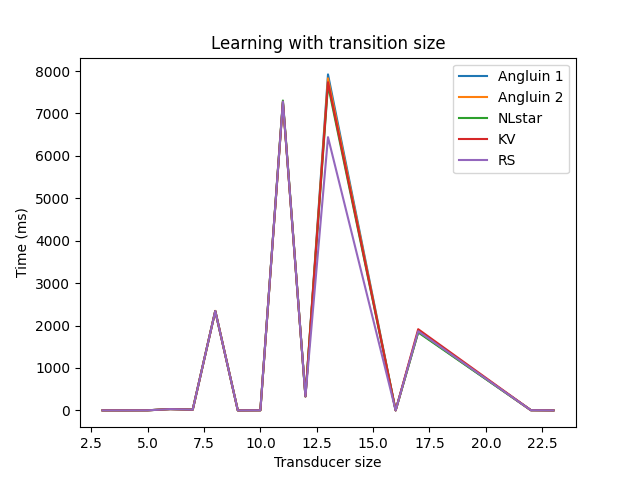
\includegraphics[scale=0.75]{figures/transition_size.png}

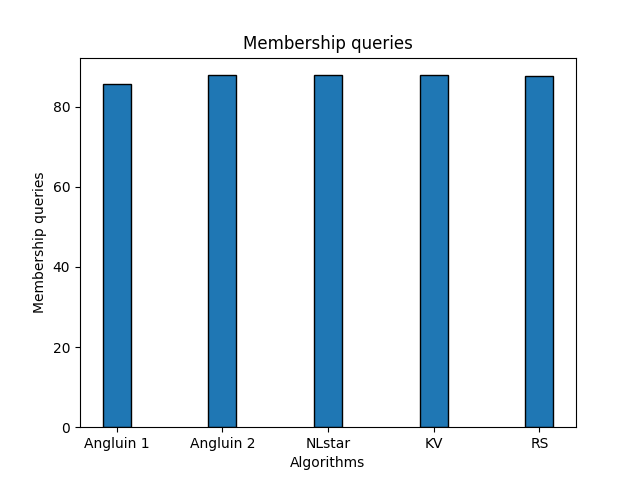
\includegraphics[scale=0.75]{figures/average_membership.png}

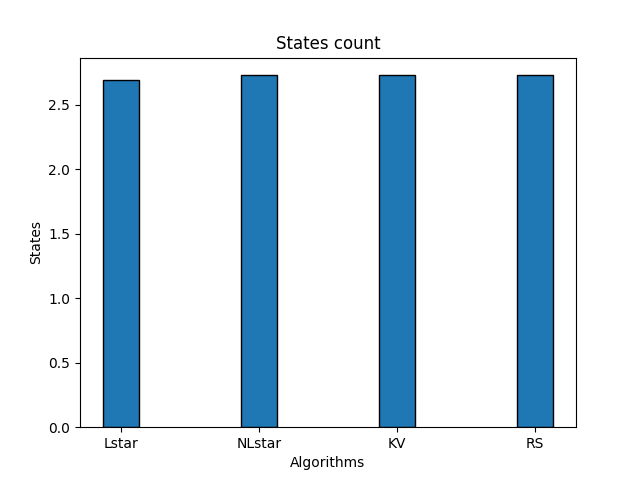
\includegraphics[scale=0.75]{figures/average_stateCount.png}